\documentclass[enabledeprecatedfontcommands, a4paper]{scrartcl}


\usepackage[ansinew]{inputenc}



\usepackage[ngerman]{babel}
\usepackage{amsmath}
\usepackage{amssymb}
\usepackage{fancyhdr}
\usepackage{color}
\usepackage{graphicx}
\usepackage{lastpage}
\usepackage{listings} 
\usepackage{tikz}
\usepackage{pdflscape}
\usetikzlibrary{trees}
\usepackage{subfigure}
\usepackage{float}
 \usepackage{polynom}
  \usepackage{hyperref}
\usepackage{tabularx}
\usepackage{forloop}
\usepackage{geometry}
\usepackage{listings}
\usepackage[]{algorithm2e}
\usepackage{fancybox}
\usepackage{tikz}
\usetikzlibrary{shapes}

\input kvmacros

%Größe der Ränder setzen
\geometry{a4paper,left=3cm, right=3cm, top=3cm, bottom=3cm}

%Kopf- und Fußzeile
\pagestyle {fancy}
\fancyhead[L]{Tutor: Benjamin Coban}
\fancyhead[C]{Theoretische Informatik}
\fancyhead[R]{\today}

\fancyfoot[L]{}
\fancyfoot[C]{}
\fancyfoot[R]{Seite \thepage /\pageref*{LastPage} }


%Formatierung der Überschrift, hier nichts ändern
\def\header#1#2{
\begin{center}
{\Large\bf Übungsblatt #1} %Blatt eintragen

{(Abgabetermin #2)}
\end{center}
}

%Definition der Punktetabelle, hier nichts ändern
\newcounter{punktelistectr}
\newcounter{punkte}
\newcommand{\punkteliste}[2]{%
  \setcounter{punkte}{#2}%
  \addtocounter{punkte}{-#1}%
  \stepcounter{punkte}%<-- also punkte = m-n+1 = Anzahl Spalten[1]
  \begin{center}%
  \begin{tabularx}{\linewidth}[]{@{}*{\thepunkte}{>{\centering\arraybackslash} X|}@{}>{\centering\arraybackslash}X}
      \forloop{punktelistectr}{#1}{\value{punktelistectr} < #2 } %
      {%
        \thepunktelistectr & 
      } 
      #2 &  $\Sigma$ \\
      \hline
      \forloop{punktelistectr}{#1}{\value{punktelistectr} < #2 } %
      {%
        &
      } &\\ 
      \forloop{punktelistectr}{#1}{\value{punktelistectr} < #2 } %
      {%
        &
      } &\\ 
    \end{tabularx}
  \end{center}
}



\begin{document}

%Hier bitte Student 1 usw ersetzen
\begin{tabularx}{\linewidth}{m{0.2 \linewidth}X}
\begin{minipage}{\linewidth}%
%
% ----------------------- TODO ---------------------------
%Hier Namen eintragen
%
Stefan Fischer\\ 
Benjamin Neidhardt\\ 
Merle Kammer
\end{minipage} & \begin{minipage}{\linewidth}%
%
% ----------------------- TODO ---------------------------
%Die zweite Zahl durch die Anzahl der Aufgaben ersetzen
%
%
\punkteliste{1}{4} %
%
\end{minipage}\\
\end{tabularx}



% ----------------------- TODO ---------------------------
%
%Hier Nummer und Datum aktualisieren
\header{Nr. 3}{11.05.2017}



\section*{Aufgabe 1}
\subsection*{a)}
Bubblesort:\\
Beim Durchlaufen des Arrays werden die jeweiligen Nachbarelemente miteinander verglichen  und ausgetauscht. \\
Am Ende des ersten Durchlaufs befindet sich das größte Element am Ende des Arrays. Dieser Vorgang wird nun erneut gestartet, allerdings diesmal ohne das letzte Element. Danach hat man das zweitgrößte Element gefunden. Der ganze Vorgang wird nun so oft wiederholt, bis das gesamte Array sortiert ist.\\
\newline
\textbf{Pseudocode}\\
\\
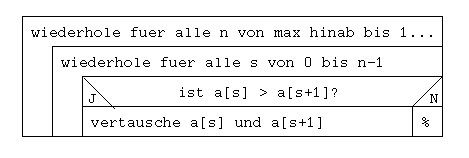
\includegraphics[width=0.50\textwidth]{Bild}\\

\noindent Beschreibung Minimumsort:\\
Beim Durchlaufen des Arrays wird das kleinste Element auf min gesetzt und mit dem ersten Element getauscht.
Am Ende des ersten Durchlaufs befindet sich das kleinste Element am Anfang des Ararys Dieser Vorgang wird nun erneut gestartet, allerdings diesmal ohne das erste  Element. Danach hat man das zweitkleinste Element gefunden. Der ganze Vorgang wird nun so oft wiederholt, bis das gesamte Array sortiert ist.

\textbf{Pseudocode}\\
\\
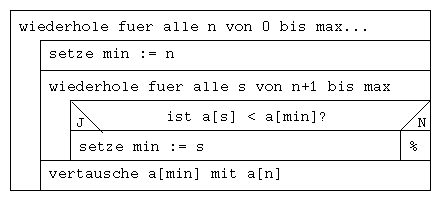
\includegraphics[width=0.50\textwidth]{Bild1}\\
\newpage
\subsection*{b)}
Bubblesort vorsortierte Liste:\\
Bei einer bereits sortierten Liste wird Bubblesort die Liste nur einmal durchgehen, um festzustellen, dass die Liste bereits sortiert ist, weil keine benachbarten Elemente vertauscht werden mussten. Daher benötigt Bubblesort   ${O}(n)$  Schritte, um eine bereits sortierte Liste zu bearbeiten.\\
Insgesamt werden also (n - 1) Vergleiche und keine Vertauschungen vorgenommen.\\
\newline
Minimum Sort vorsortiere Liste:\\
Bei einer vorsortieren Liste muss MinSort mindestens einmal alle Zahlen vergleichen.Daher benötigt auch MinSort   ${O}(n)$  Schritte, um eine bereits sortierte Liste zu bearbeiten.\\
Insgesamt werden also (n - 1) Vergleiche und keine Vertauschungen vorgenommen.\\
\newpage
\subsection*{c + d)}
Bubblesort:\\
Bei absteigend sortierten Liste wird in jedem Durchlauf der inneren Schleife das erste Element bis zum n - 1 Element durchgetauscht (also n -1 viele  Vertausch-Operationen) und der Wert von n um 1 reduziert. Da dies die maximale Anzahl an Vertausch-Operationen und Vergleichs-Operationen pro Iteration und die maximale Anzahl an Iterationen liefert, ist dies der Worst-Case mit der Laufzeit $\Theta(n^{2})$.\\

Insgesamt führt Bubble Sort also höchstens:\\

$\sum_{i=1}^{n-1} (n-i) = \sum_{j=1}^{n-1} j = \dfrac{n \cdot (n-1)}{2}$\\

Vergleiche und Vertauschungen durch.\\

Beispiel Liste absteigend sortiert:\\
\begin{array}[t]{lllrr}
  5 & 4 & 3 & 2 & 1\\
  \\
  4 & 5 & 3 & 2 & 1\\
  4 & 3 & 5 & 2 & 1\\
  4 & 3 & 2 & 5 & 1\\
  4 & 3 & 2 & 1 & 5\\
  3 & 4 & 2 & 1 & 5\\
  3 & 2 & 4 & 1 & 5\\
  3 & 2 & 1 & 4 & 5\\
  2 & 3 & 1 & 4 & 5\\
  2 & 1 & 3 & 4 & 5\\
  2 & 1 & 3 & 4 & 5\\
 \\
 1 & 2 & 3 & 4 & 5\\
  \end{array}\\
  
\noindent Berechnung der max Vergleiche:\\
\hspace*{10mm} $\dfrac{5 \cdot (5-1)}{2} = $10 Vergleiche  \\
\\
Berechnung der max Vertauschungen:\\
\hspace*{10mm} $\dfrac{5 \cdot (5-1)}{2} =$ 10 Vertauschungen  \\

\noindent Minimum Sort:\\
Beim Minimum Sort spielt der Inhalt des Eingabe-Arrays keine Rolle für die Anzahl an Vertausch-Operationen, da diese auf jeden Fall genau einmal in jeder Iteration der äußeren Schleife ausgefuührt werden und die Anzahl der Iterationen nur von der Länge des Eingabe- Arrays abhängt.\\

Insgesamt führt MinSort also höchstens:\\

$(n-1)$\\

Vergleiche und Vertauschungen durch.\\

Beispiel Liste absteigend sortiert:\\
\begin{array}[t]{lllrr}
  5 & 4 & 3 & 2 & 1\\
  \\
  1 & 4 & 3 & 2 & 5\\
  1 & 2 & 3 & 4 & 5\\
 \\
  1 & 2 & 3 & 4 & 5\\
  \end{array}\\
  
Berechnung der max Vergleiche:\\
$(n-1)= 5 -1 =$ 4 Vergleiche  \\
\\
Berechnung der max Vertauschungen:\\
$(n-1)= 5 -1 =$ 4 Vertauschungen  \\

\newpage
\section*{Aufgabe 2}
Die Laufzeit von Quicksort ist im allgemeinen gegegen durch:\\
\begin{align*} {T}(n) = {T}(k) + {T}(n-k) + {O}(n)
\end{align*}\\
wobei k das Pivotelemet ist (bzw. die Einteilung der Gruppen).\\
\newline
\noindent Damit die Eingabe stehts so geteilt wird, dass die Anzahl der kleinen Elemente doppelt so groß ist wie die der größten Elemente muss $k = \dfrac{2n}{3}$ sein!\\
Es folgt:\\
\begin{align*} {T}(n) = {T}(\dfrac{2n}{3}) + {T}(n - \dfrac{2n}{3}) + {O}(n)
                                = {T}(\dfrac{2n}{3}) + {T}(\dfrac{n}{3}) + {O}(n)
\end{align*}\\
Behauptung: ${T}(n) \le c\cdot n \cdot log \cdot n  $ für konstante c\\
Beweis:\\
${T}(n) = c \cdot \dfrac{2n}{3} \cdot log  (\dfrac{2n}{3}) + c \cdot \dfrac{n}{3} \cdot log  (\dfrac{n}{3}) + O}(n)
$\\
\\
\hspace*{8mm} $= c \cdot \dfrac{2n}{3} \cdot (log (n) - log  (\dfrac{3}{2}) + c \cdot \dfrac{n}{3} \cdot (log (n) -  log  (3)) + O}(n)
$\\
\\
\hspace*{8mm} $= c \cdot \dfrac{2n}{3} \cdot log (n) - c \cdot \dfrac{2n}{3} \cdot log (\dfrac{3}{2}) + c \cdot \dfrac{n}{3} \cdot log (n) - c \cdot \dfrac{n}{3} log  (3) + O}(n)
$\\
\\
\hspace*{8mm} $= c \cdot n \cdot log (n) - c \cdot \dfrac{n}{3} \cdot (2log(\dfrac{3}{2} + log (3)) +  O}(n)
$\\
\\
\hspace*{8mm} $= c \cdot n \cdot log (n) - c \cdot n \cdot \dfrac{1}{3} \cdot log(\dfrac{27}{4}) +  O}(n)
$\\
\\
\hspace*{8mm} $\le c \cdot n \cdot log (n)$ für $ c \cdot \dfrac{3}{log(\dfrac{27}{4})}
\approx 1.08897$\\
\\
\noindent Da in der Aufgabe steht, dass $c \in N$ müssen wir $c \cdot \dfrac{3}{log(\dfrac{27}{4})}$ runden\\ 
\noindent(aufrunden, da $\ge$ und c Mindeswert ist wir daher nicht abrunden können) \\
\rightarrow c $ \ge $ 2 muss mindestens erfüllt sein!!
\newpage

\section*{Aufgabe 3}
\subsection*{a)}
$A = \{9, 7, 21, 14, 88, 23, 10, 26, 13\}$
\\
\\
\textbf{Bilden des Heaps:}
\\
\\
\begin{figure}[h!]
Einfügen von 9
\\
\\
\ovalbox{

\begin{tikzpicture}[level/.style={sibling distance=60mm/#1}]
\node [circle,draw] (9){$9$}
;
\end{tikzpicture}}

\end{figure}

\vspace{1cm}

\begin{figure}[h!]
Einfügen von 7
\\
\\
\ovalbox{
\begin{tikzpicture}[level/.style={sibling distance=60mm/#1}]
\node [circle,draw] (9){$9$}
child {node [circle,draw] (a) {$7$}}
;
\end{tikzpicture}}
\end{figure}

\begin{figure}[h!]
Wiederherstellen des Heap mit Beachtung des Kriteriums
\\
\\
\ovalbox{
\begin{tikzpicture}[level/.style={sibling distance=60mm/#1}]
\node [circle,draw] (9){$7$}
child {node [circle,draw] (a) {$9$}}
;
\end{tikzpicture}}
\end{figure}
\vspace{2cm}

\begin{figure}[h!]

Einfügen von 21
\\
\\
\ovalbox{
\begin{tikzpicture}[level/.style={sibling distance=60mm/#1}]
\node [circle,draw] (9){$7$}
child {node [circle,draw] (a) {$9$}}
child {node [circle,draw] (b) {$21$}}
;
\end{tikzpicture}}
\end{figure}
\vspace{1cm}

\begin{figure}[h!]
Einfügen von 14
\\
\\
\ovalbox{
\begin{tikzpicture}[level/.style={sibling distance=60mm/#1}]
\node [circle,draw] (9){$7$}
	child {node [circle,draw] (a) {$9$}
		child {node [circle,draw] (c) {$14$}}
}
child {node [circle,draw] (b) {$21$}}
;
\end{tikzpicture}}
\end{figure}
\vspace{1cm}

\begin{figure}[h!]
Einfügen von 88
\\
\\
\ovalbox{
\begin{tikzpicture}[level/.style={sibling distance=60mm/#1}]
\node [circle,draw] (9){$7$}
	child {node [circle,draw] (a) {$9$}
		child {node [circle,draw] (c) {$14$}}
		child {node [circle,draw] (d) {$88$}}
}
child {node [circle,draw] (b) {$21$}}
;
\end{tikzpicture}}
\end{figure}
\vspace{1cm}

\begin{figure}[h!]
Einfügen von 23
\\
\\
\ovalbox{
\begin{tikzpicture}[level/.style={sibling distance=60mm/#1}]
\node [circle,draw] (9){$7$}
	child {node [circle,draw] (a) {$9$}
		child {node [circle,draw] (c) {$14$}}
		child {node [circle,draw] (d) {$88$}}
}
child {node [circle,draw] (b) {$21$}
		child {node [circle,draw] (c) {$23$}}
		}
;
\end{tikzpicture}}
\end{figure}
\vspace{1cm}

\begin{figure}[h!]
Einfügen von 10
\\
\\
\ovalbox{
\begin{tikzpicture}[level/.style={sibling distance=60mm/#1}]
\node [circle,draw] (9){$7$}
	child {node [circle,draw] (a) {$9$}
		child {node [circle,draw] (c) {$14$}}
		child {node [circle,draw] (d) {$88$}}
}
child {node [circle,draw] (b) {$21$}
		child {node [circle,draw] (c) {$23$}}
		child {node [circle,draw] (c) {$10$}}
		}
;
\end{tikzpicture}}
\end{figure}
\vspace{1cm}

\begin{figure}[h!]
Wiederherstellen des Heap mit Beachtung des Kriteriums
\\
\\
\ovalbox{
\begin{tikzpicture}[level/.style={sibling distance=60mm/#1}]
\node [circle,draw] (9){$7$}
	child {node [circle,draw] (a) {$9$}
		child {node [circle,draw] (c) {$14$}
		}
		child {node [circle,draw] (d) {$88$}}
}
child {node [circle,draw] (b) {$10$}
		child {node [circle,draw] (c) {$23$}}
		child {node [circle,draw] (c) {$21$}}
		}
;
\end{tikzpicture}}
\end{figure}
\vspace{1cm}

\begin{figure}[h!]
Einfügen von 26
\\
\\
\ovalbox{
\begin{tikzpicture}[level/.style={sibling distance=60mm/#1}]
\node [circle,draw] (9){$7$}
	child {node [circle,draw] (a) {$9$}
		child {node [circle,draw] (c) {$14$}
		child {node [circle,draw] (d) {$26$}}
		}
		child {node [circle,draw] (d) {$88$}}
}
child {node [circle,draw] (b) {$10$}
		child {node [circle,draw] (c) {$23$}}
		child {node [circle,draw] (c) {$21$}}
		}
;
\end{tikzpicture}}
\end{figure}
\vspace{1cm}

\begin{figure}[h!]
Einfügen von 13
\\
\\
\ovalbox{
\begin{tikzpicture}[level/.style={sibling distance=60mm/#1}]
\node [circle,draw] (9){$7$}
	child {node [circle,draw] (a) {$9$}
		child {node [circle,draw] (c) {$14$}
		child {node [circle,draw] (d) {$26$}}
		child {node [circle,draw] (d) {$13$}}
		}
		child {node [circle,draw] (d) {$88$}}
}
child {node [circle,draw] (b) {$10$}
		child {node [circle,draw] (c) {$23$}}
		child {node [circle,draw] (c) {$21$}}
		}
;
\end{tikzpicture}}
\end{figure}
\vspace{1cm}

\begin{figure}[h!]
Wiederherstellen des Heap mit Beachtung des Kriteriums
\\
\\
\ovalbox{
\begin{tikzpicture}[level/.style={sibling distance=60mm/#1}]
\node [circle,draw] (9){$7$}
	child {node [circle,draw] (a) {$9$}
		child {node [circle,draw] (c) {$13$}
		child {node [circle,draw] (d) {$26$}}
		child {node [circle,draw] (d) {$14$}}
		}
		child {node [circle,draw] (d) {$88$}}
}
child {node [circle,draw] (b) {$10$}
		child {node [circle,draw] (c) {$23$}}
		child {node [circle,draw] (c) {$21$}}
		}
;
\end{tikzpicture}}
\end{figure}
\vspace{1cm}
\\
¥\subsection*{b)}
EXTRACTMIN Operation ausführen und Heap-Eigenschaft wiederherstellen:
\\
\begin{figure}[h!]
\ovalbox{
\begin{tikzpicture}[level/.style={sibling distance=60mm/#1}]
\node [circle,draw] (9){$7$}
	child {node [circle,draw] (a) {$9$}
		child {node [circle,draw] (c) {$13$}
		child {node [circle,draw] (d) {$26$}}
		child {node [circle,draw] (d) {$14$}}
		}
		child {node [circle,draw] (d) {$88$}}
}
child {node [circle,draw] (b) {$10$}
		child {node [circle,draw] (c) {$23$}}
		child {node [circle,draw] (c) {$21$}}
		}
;
\end{tikzpicture}}
\end{figure}
\\
\\
\\
\\
Entnehme das Minimum d.h. die Wurzel des Baumes und füge 14 als neue Wurzel hinzu:
\\
\begin{figure}[h!]
\ovalbox{
\begin{tikzpicture}[level/.style={sibling distance=60mm/#1}]
\node [circle,draw] (9){$14$}
	child {node [circle,draw] (a) {$9$}
		child {node [circle,draw] (c) {$13$}
		child {node [circle,draw] (d) {$26$}}
		}
		child {node [circle,draw] (d) {$88$}}
}
child {node [circle,draw] (b) {$10$}
		child {node [circle,draw] (c) {$23$}}
		child {node [circle,draw] (c) {$21$}}
		}
;
\end{tikzpicture}}
\end{figure}
\\
\\
Vergleiche 14 mit beiden Kindelementen und tausche mit kleinerem, also der 9:
\\
\begin{figure}[h!]
\ovalbox{
\begin{tikzpicture}[level/.style={sibling distance=60mm/#1}]
\node [circle,draw] (9){$9$}
	child {node [circle,draw] (a) {$14$}
		child {node [circle,draw] (c) {$13$}
		child {node [circle,draw] (d) {$26$}}
		}
		child {node [circle,draw] (d) {$88$}}
}
child {node [circle,draw] (b) {$10$}
		child {node [circle,draw] (c) {$23$}}
		child {node [circle,draw] (c) {$21$}}
		}
;
\end{tikzpicture}}
\end{figure}
\\
\\
Vergleiche 14 wieder mit beiden Kindelementen, falls kleiner, tausche mit dem kleinsten, in dem Fall der 13:
\begin{figure}[h!]
\ovalbox{
\begin{tikzpicture}[level/.style={sibling distance=60mm/#1}]
\node [circle,draw] (9){$9$}
	child {node [circle,draw] (a) {$13$}
		child {node [circle,draw] (c) {$14$}
		child {node [circle,draw] (d) {$26$}}
		}
		child {node [circle,draw] (d) {$88$}}
}
child {node [circle,draw] (b) {$10$}
		child {node [circle,draw] (c) {$23$}}
		child {node [circle,draw] (c) {$21$}}
		}
;
\end{tikzpicture}}
\end{figure}
\\
Dies ist der finale Heap, da die Heap-Eigenschaft nun komplett wiederhergestellt ist.
\\
\\
\\
\\
\\
\\
\\
\\
\\
\\
\\
\\
\\
\\
\subsection*{c)}
Neues Element 6 zu Heap hinzufügen:
\begin{figure}[h!]
\ovalbox{
\begin{tikzpicture}[level/.style={sibling distance=60mm/#1}]
\node [circle,draw] (9){$9$}
	child {node [circle,draw] (a) {$13$}
		child {node [circle,draw] (c) {$14$}
		child {node [circle,draw] (d) {$26$}}
		child {node [circle,draw] (d) {$6$}}
		}
		child {node [circle,draw] (d) {$88$}}
}
child {node [circle,draw] (b) {$10$}
		child {node [circle,draw] (c) {$23$}}
		child {node [circle,draw] (c) {$21$}}
		}
;
\end{tikzpicture}}
\end{figure}
\vspace{1cm}
\\
\\
Heap-Eigenschaft nach und nach wiederherstellen:

\begin{figure}[h!]
\ovalbox{
\begin{tikzpicture}[level/.style={sibling distance=60mm/#1}]
\node [circle,draw] (9){$9$}
	child {node [circle,draw] (a) {$13$}
		child {node [circle,draw] (c) {$6$}
		child {node [circle,draw] (d) {$26$}}
		child {node [circle,draw] (d) {$14$}}
		}
		child {node [circle,draw] (d) {$88$}}
}
child {node [circle,draw] (b) {$10$}
		child {node [circle,draw] (c) {$23$}}
		child {node [circle,draw] (c) {$21$}}
		}
;
\end{tikzpicture}}
\end{figure}
\vspace{1cm}

\begin{figure}[h!]
\ovalbox{
\begin{tikzpicture}[level/.style={sibling distance=60mm/#1}]
\node [circle,draw] (9){$9$}
	child {node [circle,draw] (a) {$6$}
		child {node [circle,draw] (c) {$13$}
		child {node [circle,draw] (d) {$26$}}
		child {node [circle,draw] (d) {$14$}}
		}
		child {node [circle,draw] (d) {$88$}}
}
child {node [circle,draw] (b) {$10$}
		child {node [circle,draw] (c) {$23$}}
		child {node [circle,draw] (c) {$21$}}
		}
;
\end{tikzpicture}}
\end{figure}
\vspace{1cm}

\begin{figure}[h!]
\ovalbox{
\begin{tikzpicture}[level/.style={sibling distance=60mm/#1}]
\node [circle,draw] (9){$6$}
	child {node [circle,draw] (a) {$9$}
		child {node [circle,draw] (c) {$13$}
		child {node [circle,draw] (d) {$26$}}
		child {node [circle,draw] (d) {$14$}}
		}
		child {node [circle,draw] (d) {$88$}}
}
child {node [circle,draw] (b) {$10$}
		child {node [circle,draw] (c) {$23$}}
		child {node [circle,draw] (c) {$21$}}
		}
;
\end{tikzpicture}}
\end{figure}
\vspace{1cm}
\pagebreak
\subsection*{d)}

Schritte in O-Notation um maximales Element aus dem Heap zu löschen?
\\
$\rightarrow$ man vergleicht alle Blätter, aber nicht die Elternknoten, da diese nach der Heap-Eigenschaft nicht das größte Element sein können
\\
\\
Schritt 1: Das Maximum finden $\rightarrow$  $[\frac{n}{2}]$ mit n Anzahl der Elemente d.h. O($[\frac{n}{2}]$)
\\
\\
Schritt 2: Maximum an unterstes Blatt,, welches am weitesten rechts steht $\rightarrow$ O(1)
\\
\\
Schritt 3: Heap-Eigenschaft wiederherstellen: max O($\log n$), da Höhe von Baum ausgewogen
\\
\\
Schritt 4: Maximum aus Baum entfernen (Heap-Eigenschaft bleibt durch Schritt 1 immer erhalten) 
\\
\\
$\rightarrow$ $[\frac{n}{2}] + 1 + \log n + 1 = [\frac{n}{2}] +\log n + 2$ $\rightarrow$ O(n)
\newpage
\section*{Aufgabe 4}
$\Omega = \{1, 2, 3, 4, 5, 6\}$
\subsection*{a)}
\begin{itemize}
\item[(a)] 
Die Wahrscheinlichkeit für das Ereignis $A=\{2\}$ ist: $P(A)=\frac{|A|}{|\Omega|}=\frac{1}{6}$
\item[(b)]
Die Wahrscheinlichkeit für das Ereignis $A=\{2, 4, 6\}$ ist: $P(A)=\frac{|A|}{|\Omega|}=\frac{3}{6}$
\end{itemize}
\subsection*{b)}
Zu zeige: Falls $A \cap B = \emptyset$, dann gilt $P(A \cap B)=P(A)+P(B)$\\
(1)
\begin{align*}
P(A \cup B) &\overset{(*)}{=} P((A \setminus B) \dot\cup (A \cap B) \dot\cup (B \setminus A))\\
&= P(A \setminus B) + P(A \cap B) + P(B \setminus A) \ \ \leftarrow \sigma \textrm{-additivität}\\
&= \underbrace{P(A \setminus B) + P(A \cap B)}_{= P(A)} + \underbrace{P(B \setminus A) + P(A \cap B)}_{=P(B)} - P(A \cap B)\\
&= P(A) + P(B) + P(A \cap B)\\
&\textrm{für $A \cap B = \emptyset$ gilt somit}\\
&= P(A) + P(B) \hspace{7cm} \Box
\end{align*}
(*):\\
$A \cup B = (A \setminus B) \dot\cup (A \cap B) \dot\cup (B \setminus A)$\\

\begin{tikzpicture}[fill=gray]
% left hand
\scope
\clip (-2,-2) rectangle (2,2)
      (1,0) circle (1);
\fill[blue!20] (0,0) circle (1);
\endscope
% right hand
\fill[blue!40] (1,0)circle (1);
\scope
\clip (-2,-2) rectangle (2,2)
      (0,0) circle (1);
\fill[blue!20] (1,0) circle (1);
\endscope
% outline
\draw (0,0) circle (1) (-0.5,0)  node [text=black,below] {$A\setminus B$}
	(0,0) circle (1) (0.5, 1.5) node[text=black, below] {$A \cup B$}
      (1,0) circle (1) (1.5,0)  node [text=black,below] {$B \setminus A$}
      (1,0) circle (1) (0.5, 0) node[text=black, above]{$A \cap B$}
      (-2,-2) rectangle (3,2) node [text=black,above] {$\Omega$};
\end{tikzpicture}\\
\\
Für $A \cap B \neq \emptyset$ gilt $P(A \cup B) \le P(A)+P(B)$ denn:\\
$P(A \cup B)=P(A) +P(B) - P(A \cap B) \leftarrow$ siehe Beweis (1)\\
$\Rightarrow P(A \cup B) \le P(A)+P(B)$
\subsection*{c)}
$\Omega = \{1, 2, 3, 4, 5, 6\}^3$\\
Das Ereignis, dass "Alle drei Würfel ein Auge zeigen ist $A=\{(1, 1, 1)\}$. Die Wahrscheinlichkeit für dieses Ereignis ist: $P(A)=P(\{(1, 1, 1)\})=\frac{|\{(1, 1, 1)\}|}{|\Omega|}= \frac{1}{6^3}=\frac{1}{216}$
\newpage
\subsection*{d)}
$\Omega = \{1, 2, 3, 4,5 ,6\}^2$
\begin{itemize}
\item[(a)]
\begin{align*}
[X=4]&=\{(x,y) \in \Omega \ | \ X(x,y)=4\}\\
&=\{(4,4),(4,5),(5,4),(4,6),(6,4)\}
\end{align*}
Es werden zwei Würfel geworfen. Das Ereignis $[X=4]$ tritt ein, wenn einer der Würfel eine 4 zeigt und die Augenzahl des anderen Würfels $\ge 4$ ist. Das heißt das Minimum der gewürfelten Augenzahlen muss 4 sein, damit das Ereignis $[X=4]$ eintrifft.
\item[(b)]
$P([X=4])=P(\{(4,4),(4,5),(5,4),(4,6),(6,4)\})=\frac{|\{(4,4),(4,4),(4,5),(5,4),(4,6),(6,4)\}|}{|\Omega|}=\frac{6}{6^2}=\frac{6}{36}=\frac{1}{6}$\\
Unter Annahme der Gleichverteilung der Ereignisse ist $P([X=4])=\frac{1}{6}$.
\end{itemize}

\end{document}
